\chapter{Sidekick Protocol}
\label{sec:sidekick}

In this paper, we propose a method for in-network assistance of opaque transport
protocols that tries to resolve this tension. Our approach leaves the transport
protocol unchanged on the wire: a secure end-to-end connection between hosts,
opaque to middleboxes and free to evolve. No PEPs are credentialed to decrypt
the transport protocol's headers.

Instead, we propose a second protocol to be spoken on an adjacent connection
between an end host and a PEP. We call this the \emph{\bf Sidekick protocol},
and its contents are \emph{about} the packets of the underlying, or ``base,''
connection. Sidekick PEPs assist end hosts by reporting what they've observed
about the packets of the opaque base connection, without coupling their
assistance to the details of the base protocol. End hosts use this information
to influence decisions about how and when to send or resend packets on the base
connection, approximating some of the performance benefits of traditional PEPs.
A similar functional separation was first proposed by \cite
{yuan2022sidecar}, but this paper presents the first concrete realization of
the idea and its nuanced interactions with real transport protocols.

One key technical challenge with this approach is how the Sidekick can
efficiently refer to ranges of packets in an opaque base connection. These
packets appear random to the middlebox, and referring to a range of, e.g., 100
opaque packets in the presence of loss and reordering is not as simple as
saying ``up to 100'' when there are cleartext sequence numbers. In \Cref
{sec:quack}, we present and evaluate a mathematical tool called a \emph
{\bf quACK} that concisely represents a selective acknowledgment of opaque,
randomly identified packets. The quACK is based on the insight that we can
model the problem as a system of power sum polynomial equations if there is a
practical bound on the maximum number of ``holes'' among the packets being
ACKed. We created an optimized implementation~\cite{quack-github}, building on
related theoretical work~\cite
{eppstein2011straggler,minsky2003set,karpovsky2003data}.

A second challenge is how the end host should use information from a Sidekick
connection to obtain a performance benefit for its base connection. Since the
performance benefit comes from changing behavior at the end host rather than
the middlebox, transport protocols need to incorporate this information into
their existing algorithms for, e.g., loss detection and retransmission, which
have gotten increasingly complex over time. To explore this, we designed a
Sidekick protocol we call Robin, and implemented it in three scenarios:
\begin{itemize}[noitemsep,topsep=2pt]
\item A low-latency audio stream over an Internet path that includes a Wi-Fi path segment
  (low latency with loss), followed by a WAN path segment (higher latency
  with low loss). Can the Sidekick PEP reduce the de-jitter buffer delay
  by triggering earlier retransmissions on loss?

\item An upload over the same path. Can an opaque transport protocol like QUIC,
  aided by a Sidekick PEP at the point between these two path segments, match
  the throughput of TCP over a connection-splitting PEP?

\item A battery-powered receiver, downloading data from the Internet over Wi-Fi.
  If the Wi-Fi access point sends Sidekick quACKs on behalf of the receiver,
  can it reduce the number of times the receiver's radio needs to wake up
  to send an end-to-end ACK?
\end{itemize}

\smallskip

A third technical challenge is how knowledge about \emph{where}
loss occurs along a path should influence a congestion-control scheme.
The challenge in any such scheme is how to maximize the congestion window
while sharing the network fairly with competing flows.
We present a path-aware modification to the CUBIC congestion-control
algorithm~\cite{ha2008cubic}, which we call \mbox{\textbf{PACUBIC}},
that approximates the congestion-control behavior of a PEP-assisted split TCP
CUBIC connection while making its decisions entirely on the host.

\paragraph{Summary of results.}

We implemented Robin in a low-latency media client
based on the WebRTC standard, and an HTTP/3 client using the Cloudflare
implementation of QUIC~\cite{quiche} and the \texttt{libcurl}~\cite{libcurl}
implementation of HTTP/3. We evaluated the three scenarios in
real-world and emulation experiments.
In real-world experiments using an unmodified local Wi-Fi network to access our
nearest AWS datacenter, the Sidekick was able to trigger early retransmissions
to fill in gaps in the audio of a latency-sensitive audio stream, reducing the
receiver's de-jitter delay from 2.3~seconds to 204~ms---about a 91\% reduction
(\Cref{fig:real-world}). The Sidekick was also able to improve the speed of an
HTTP/3 (QUIC) upload by about 50\%.

In emulation experiments of the ``battery-powered receiver'' scenario,
the Sidekick PEP was able to reduce the need for the receiver to send ACKs
by sending proxy acknowledgments on its behalf---ACKs the sender used
to advance its flow-control and congestion-control windows. The
receiver only needed to wake up its radio to send occasional
end-to-end ACKs, which the sender used to discard data from its
buffer (\Cref{fig:ack-reduction}).

Also in an emulation experiment, we confirmed that PACUBIC's
performance approximates a split CUBIC connection (two TCP CUBIC
connections separated by a PEP), responding to loss events on the
different path segments similarly to how the individual CUBIC flows would
(\Cref{fig:loss-vs-tput}). The results indicate that the Sidekick protocol's gains
do not come at the
expense of congestion-control fairness relative to a split CUBIC connection.

\smallskip

The rest of this paper describes the Sidekick's motivating scenarios
(\Cref{sec:sidekick:motivating}), discusses the concrete Sidekick protocol we
built around quACKs (\Cref{sec:sidekick:protocol}) and its implementation in two
base protocols (\Cref{sec:sidekick:implementation}), and then evaluates the
protocol in real-world and emulation experiments
(\Cref{sec:sidekick:evaluation}).

\section{Motivating Scenarios}
\label{sec:sidekick:motivating}

\begin{figure}[t]
	\centering
	% \includegraphics[width=\linewidth]{figures/sc-legend.pdf}\\
	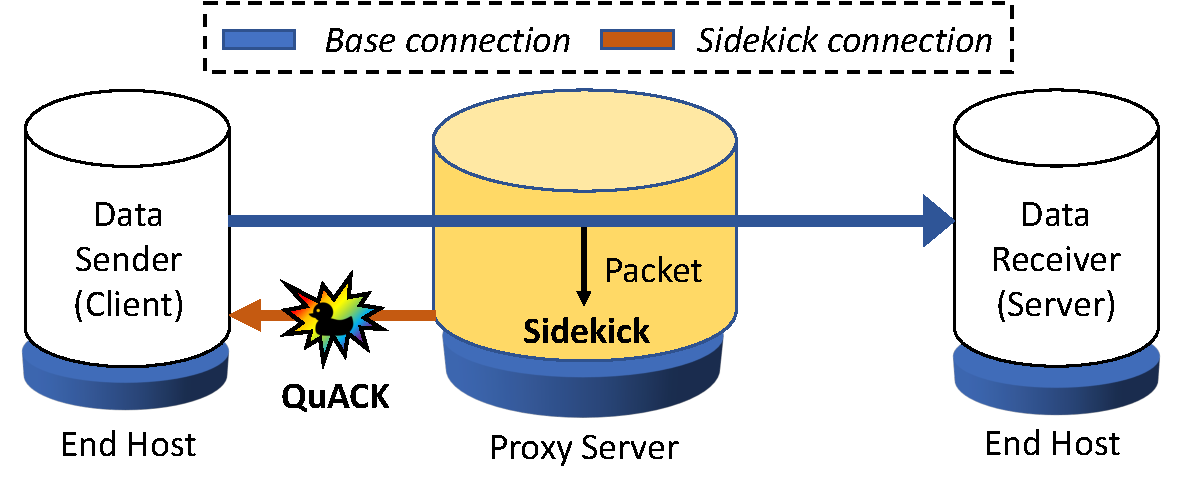
\includegraphics[width=\linewidth]{figures/sc_protocol.pdf}%
\caption{The proxy generates quACKs, in-network acknowledgments, based on
the opaque packets it observes in the base protocol. It quACKs to an end
host, the data sender, which sends or resends packets on the base protocol as a result.
Although we only show one side of the connection, the \sys could assist
either end host of a bidirectional flow.
\vspace{-0.4cm}
}
\label{fig:sc-protocols}
\end{figure}


We focus on three scenarios where end hosts benefit from in-network assistance.
In each one, a proxy server provides feedback, called a quACK, to an end host:
the data sender (\Cref{fig:sc-protocols}). Recall that a quACK is a
``cumulative ACK + selective ACK'' over encrypted sequence numbers. The data
sender uses this feedback to influence its behavior on the base connection,
without altering the wire format.

To be clear: the Sidekick protocol is not tied to a specific base protocol
nor to how the end hosts use the quACK information. The base protocol does not
need to be reliable, nor to have unique datagrams---we implemented and evaluated
the same Sidekick protocol and the same middlebox behavior across the different
scenarios in this paper.

\paragraph{Low-Latency Media.}

Consider a train passenger using on-board Wi-Fi to have a low-latency audio
conversation, using WebRTC/SRTP~\cite{rfc8834webrtc}, with a friend. The
end-to-end network path contains a low-latency, high-loss ``near'' path
segment (the Wi-Fi hop) followed by a high-latency, low-loss ``far'' path
segment (the cellular and wired path over the Internet). The friend probably
suffers from poor connection quality, experiencing drops in the audio stream or
high de-jitter buffer delays from waiting for retransmitted packets to be
played in order (\Cref{fig:media} in emulation, \Cref
{fig:real-world:scenario1} in real world).

In the Sidekick approach, a Sidekick on the Wi-Fi access point sends quACKs to the audio
application on the user's laptop, assisting the base connection's data sender.
The sender uses quACKs to retransmit packets sooner than they would have using
negative acknowledgments (NACKs) from the receiver. The end result is similar
to the effect of prior PEPs, such as Snoop~\cite{balakrishnan1995snoop} and
Milliproxy~\cite{polese2017milliproxy}, that leverage TCP's cleartext sequence
numbers to trigger early retransmission on lossy wireless paths.

\paragraph{Connection-Splitting PEP Emulation.}

Consider the same train passenger as before but uploading a large file over the
Internet with a reliable transport protocol. If the protocol were TCP, the
train could deploy a split TCP PEP at the access point. The split connection
allows quick detection and retransmission of dropped packets on the lossy Wi-Fi
segment, while opening up the congestion window on the high-latency cellular
segment.

However, opaque transport protocols like QUIC can't benefit from (nor be harmed
by) connection-splitting PEPs. Without a PEP, QUIC relies on end-to-end
mechanisms over the entire path to detect losses, recover from them, and adjust
the congestion-control behavior. This leads to reduced upload speeds
(\Cref{fig:baseline-line} in emulation, \Cref{fig:real-world:scenario2} in real world).

With help from the same Sidekick PEP, the QUIC sender combines information from
quACKs and end-to-end ACKs to emulate the congestion-control behavior of a
split TCP connection (\Cref{sec:sidekick:protocol:sender-behavior}). The
application considers whether packets are lost on the near or far path
segments, and adjusts the congestion window accordingly while respecting the
opacity of the end-to-end base connection. The application also retransmits the
packet as soon as the loss has been detected.

The only guarantee the proxy makes to the sender via the quACK is that it has
received some packets. To respect the end-to-end reliability contract with the
receiver, the sender does not delete packets that may need to be transmitted
until it receives an ACK, even if the packet has been quACKed.

\paragraph{ACK Reduction.}

Now consider a battery-powered device downloading a large file from the
Internet. To reduce how often the receiver's
radio needs to wake up, saving energy, the base connection can reduce the
frequency of end-to-end ACKs the device sends.
ACK reduction has also been shown to improve performance by reducing collisions
and contention over half-duplex links~\cite{custura2023reducing,li2020tack}.
The ACK frequency can be configured with a TCP kernel setting or proposed
QUIC extension~\cite{ietf-quic-ack-frequency-07}.

However, ACK reduction can also degrade throughput~\cite{custura2023reducing,custura2020impact}
(\Cref{fig:ack-reduction} in emulation).
The sender receives more delayed feedback about loss, and has to carefully
pace packets to avoid bursts in the large delay between ACKs.
One proposal has the PEP acknowledge packets on behalf of the
receiver~\cite{kliazovich2012arqproxy}, leveraging cleartext TCP sequence
numbers, but it does not apply to opaque transport protocols.

In this case, a Sidekick at the Wi-Fi access point (or a cellular base station)
quACKs to the sender on behalf of the receiver. The receiver still occasionally
wakes up its radio to send ACKs, but the sender uses the more frequent quACKs
to advance its flow-control and congestion-control windows.

The sender respects the end-to-end reliability contract by only deleting packets
in response to ACKs, but disregards the receiver's flow control by using quACKs
to advance the flow-control window. If the sender only used ACKs to advance the
window, it would waste time waiting between ACKs to send packets with too small
a window, and need to pace sent packets on receiving a large ACK with too large
a window.

\section{Sidekick Protocol}
\label{sec:sidekick:protocol}

\paragraph{Configuration Messages.}

The data sender can send various other messages to the proxy
to configure the connection or reset bad state.

\paragraph{Resets.}
Robin allows the sender to tell the PEP to reinitialize the quACK.
This is helpful if the quACK becomes
invalid, e.g., if $m$ exceeds the threshold $t$. It is
always safe to reset the quACK, or even to ignore the Sidekick entirely and
fall back to the base protocol's end-to-end mechanisms.

\subsection{Handshake}
\label{sec:sidekick:protocol:handshake}

Sidekick connections can be configured explicitly or implicitly.  In systems that
explicitly configure proxies, such as Apple's iCloud Private Relay~\cite{icloud-private-relay}
based on MASQUE~\cite{kosek2021masque,kramer2021masquepep}, proxies can simply negotiate
sending quACKs during session establishment.  In most other settings,
such as 4G/5G cellular networks, PEPs have traditionally been deployed
as transparent proxies, silently interposing on end-to-end
connections.  Senders therefore need a way to detect transparent Sidekick
proxies and inform them of where to send quACKs.  Because of network
address translation, all communication to the proxy must be initiated
by the sender or use the same IP addresses and port numbers of the
base connection.

Our current design has senders signal quACK support by sending a
distinguished packet containing a 128-byte \emph{Sidekick-request} marker.  Such
inline signaling could confuse receivers, but Sidekicks target
protocols such as QUIC that discard cryptographically unauthenticated
data anyway.  It would be cleaner to signal support through
out-of-band UDP options~\cite{ietf-tsvwg-udp-options-28}, which we hope to do
once they are standardized.

The proxy replies to a Sidekick-request packet by sending a special packet
from the receiver's IP address and port number back to the sender.
This packet contains a \emph{Sidekick-reply} marker, an opaque session ID, and an
IP address and port number for communicating with the proxy.  Upon
receiving the Sidekick-reply packet, the sender begins communicating
directly with the proxy from a different UDP port.  It initially sends
back the session ID and configuration parameters to start receiving
quACKs.

\paragraph{Security.}
A malicious third-party could execute a reflection amplification attack that
generates a large amount of traffic while hiding its source. This is
possible because the sender requests quACKs to a different port and (for some
carrier-grade NATs) IP address from the underlying session. To mitigate this,
each quACK contains a quota, initially 1, of remaining quACKs the proxy will
send as well as an updated session ID\@.
The quota and session ID ensure only the sender can increase the quota or
otherwise reconfigure the session.

An adversarial PEP could send misleading information to the sender. Note that
only on-path PEPs can send credible information, since they refer to unique
packet identifiers.
To mitigate this, the sender can consider PEP feedback along with
end-to-end metrics to determine whether to keep using the PEP. The sender can
always opt out of the PEP, and the PEP cannot actively manipulate traffic any
more than outside a Sidekick setting.

\paragraph{Protocol parameters.}
The sender configures (i) the quACK interval of the PEP and (ii) the threshold
number of missing packets $t$, or otherwise selects Sidekick-specific settings
such as how an identifier is computed.

The quACK interval is expressed in terms of time or number of packets,
 e.g., every $N$ milliseconds or every $N$ packets, as in a TCP delayed ACK.
The sender determines the desired interval based on its estimated
RTT of the base connection and its application objectives, e.g.,
more frequently for latency-sensitive applications or lower-RTT paths.

The threshold represents the bound on the number of missing packets
between quACKs, in practice the number of ``holes'' among the packets that are
selectively ACKed. The threshold depends on the quACK interval, and
should be set based on how precise loss detection needs to be and
other qualities of the link.
For example, the threshold is larger to detect congestive loss in the queue of a
bottleneck link, or smaller to still detect transmission error on a lossy link.

\newtcolorbox{protopayload}[2][]{
  colback=yellow!20,
  colframe=black,
  boxrule=0.5pt,
  arc=1pt,
  fontupper=\ttfamily,
  width=\linewidth,
  fonttitle=\small\bfseries,
  top=-1.5mm,
  bottom=-1.5mm,
  left=2mm,
  right=2mm,
  title={#2},
  #1
}

\begin{figure}[t]
    % \centering
    % Client payloads
    \begin{subfigure}[b]{0.48\linewidth}
        \begin{protopayload}{\texttt{Init}}
            \begin{lstlisting}[language=Rust,basicstyle=\footnotesize]
epoch: u32;
base_conn: [u8; 12];
eack_ty: u8;
num_symbols: u8;
id_offset: u16;
mem_bytes: u32;
            \end{lstlisting}
        \end{protopayload}
        \begin{protopayload}{\texttt{quACK}}
            \begin{lstlisting}[language=Rust,basicstyle=\footnotesize]
count: u32;
last_identifier: u32;
code: Vec<Symbol>;
            \end{lstlisting}
        \end{protopayload}
        \caption{Client payloads.}
        \label{fig:payloads:client}
    \end{subfigure}
    \hfill
    % Proxy payloads
    \begin{subfigure}[b]{0.48\linewidth}
        \begin{protopayload}{\texttt{InitACK}}
            \begin{lstlisting}[language=Rust,basicstyle=\footnotesize]
epoch: u32;
udp_port: u16;
errno: u32;
            \end{lstlisting}
        \end{protopayload}
        \begin{protopayload}{\texttt{Reset}}
            \begin{lstlisting}[language=Rust,basicstyle=\footnotesize]
epoch: u32;
errno: u32;
            \end{lstlisting}
        \end{protopayload}
        \begin{protopayload}{\texttt{Retransmit}}
            \begin{lstlisting}[language=Rust,basicstyle=\footnotesize]
udp_payload: Vec<u8>;
            \end{lstlisting}
        \end{protopayload}
        \caption{Proxy payloads.}
        \label{fig:payloads:proxy}
    \end{subfigure}
  % Caption
  \caption{Packrat protocol messages to initialize the connection and generate
   retransmissions. There are two constructions of the quACK: power sum and
   IBLT (\Cref{sec:quack}). The \texttt{Symbol} uses 5 and 4 bytes in each
   type, respectively.}
  \label{fig:payloads}
\end{figure}


\paragraph{Payloads.} Now we describe the messages that are exchanged in the
Packrat protocol (\Cref{fig:payloads}), starting with the handshake.

Packrats are distinguished from other types of proxies such as VPNs and
transparent PEPs in that the proxy is on the path and the client is knowingly
receiving in-network retransmissions. In order to discover Packrat proxies on the
path, the client sends a magic discovery packet along the base connection
4-tuple, after it has established that connection. Proxies respond by
announcing that they support Packrat and their supported configurations, and the
server discards the invalid magic packet. Clients can choose to accept
assistance from a proxy by replying with an \texttt{Init} and their
configuration request. The proxy completes the handshake with an \texttt
{InitACK} and a new UDP address specific to this base connection.

The client configuration in \texttt{Init} includes several parameters (\Cref
{fig:payloads:client}). This includes: the type of encoding used for the quACK,
the number of symbols to use in the encoding, the byte offset in the randomly
encrypted payload at which to parse the 4-byte identifier, and the size of the
requested cache. The client may dynamically adjust these configurations with
new \texttt{Init} packets as it learns more about the network path.

The proxy accepts or rejects these configurations with an \texttt{InitACK}, and
is ready to cache packets and retransmit. On receiving an \texttt{InitACK}, the
client is free to send quACKs.

\subsection{Proxy Behavior}
\label{sec:sidekick:protocol:proxy-behavior}

\subsection{Data Sender Behavior}
\label{sec:sidekick:protocol:sender-behavior}

In this section, we discuss two particular sender-side behaviors that are enabled by
the Sidekick protocol and which are helpful across several scenarios: detecting packet loss
from a decoded quACK and congestion control.

\subsubsection{Detecting Loss}

The sender knows definitively which packets have been received by the proxy from
a decoded quACK. Next, it must determine from the remaining packets which ones
have been dropped and which are still in-flight, including if there has been a
reordering of packets. In-flight packets are later
classified as received or dropped based on future quACKs.

When there is no reordering, the packets that are dropped are just the ``holes''
among the packets that are selectively ACKed by the quACK. In particular, these
are the holes when considering sent packets in the order they were sent up to
the last element received, which represents the last selective ACK.
To identify these dropped packets, the sender encodes $t$ cumulative power sums
of its sent packets up to the last element received.
The difference between these power sums and the power
sums in the quACK represents the dropped packets. The sender ``removes'' the
identifiers of dropped packets from its cumulative power sums, ensuring that
the only packets that contribute to the threshold limit are those that
went missing since decoding the last quACK.
%  \michael{can we, instead of ``accumulates'', say: ``locally calculates'' ? This would seem clearer. Or are you trying to
% say that this is a continuously updated number?  If so, perhaps: ``locally calculates a cumulatively updated power sum quACK ...''?}

To account for reordering in loss detection, Robin implements an algorithm
similar to the 3-duplicate ACK rule in TCP~\cite{rfc5681tcp,rfc2001tcp}.
In TCP, if three or more duplicate ACKs are received in a row, it is a strong
indication that a segment has been lost. Robin considers a packet lost only if
three or more packets sent after the missing packet have been received.
Other mechanisms could involve timeouts for individual packets similar to the
RACK-TLP loss detection algorithm for TCP~\cite{rfc8985}.

\subsubsection{Path-Aware CUBIC Congestion Control}

Congestion-controlled base protocols must have a congestion response to lost
packets that they retransmit due to quACKs, similar to if the loss were
discovered by the end-to-end ACK.
This ensures friendliness with end-to-end congestion control algorithms that do
consider the loss, such as CUBIC~\cite{ha2008cubic} in the presence of a
connection-splitting TCP PEP.
Here, we propose PACUBIC, an algorithm that emulates this ``split CUBIC''
behavior. PACUBIC uses knowledge of where loss occurs to improve connection
throughput compared to end-to-end CUBIC, while remaining fair to competing flows.

Recall that CUBIC~\cite{ha2008cubic} reduces its congestion window by a
multiplicative decrease factor,
$\beta = \beta^* = 0.7$, when observing loss (a congestion event), and otherwise increases
its window based on a real-time dependent cubic function with scaling factor
$C=C^*=0.4$:
\[
cwnd = C(T-K)^3 + w_{max} \text{ where } K = \sqrt[3]{\frac{w_{max}(1-\beta)}{C}}.
\]

\noindent Here, $cwnd$ is the current congestion window,
$w_{max}$ is the window size just before the last reduction,
and $T$ is the time elapsed since the last window reduction.

While a split CUBIC connection has \emph{two} congestion windows,
end-to-end PACUBIC only has \emph{one} window representing the in-flight bytes
of the end-to-end connection.
Conceptually, we want an algorithm that enables PACUBIC's single
congestion window to match the sum of the split connection's two congestion
windows.

PACUBIC effectively makes it so that we reduce and grow $cwnd$
proportionally to the number of in-flight bytes on the path segment
of where the last congestion event occurred.
Let $r$ be the estimated ratio of the RTT of the near path segment
(between the data sender and the proxy) to the RTT of the entire connection
(between end hosts).
We use $r$ as a proxy for the ratio of the number of in-flight bytes.
If the last congestion event came from a quACK, we use the same real-time
dependent cubic function but with the following
constants\footnote{See \Cref{sec:appendix:pacubic} for more intuition behind $\beta'$ and $C'$.}
\[
\beta = 1 - r(1-\beta^*)\text{ and }C = \frac{C^*}{r^3}.
\]
\noindent If the last congestion event came from an end-to-end ACK, then we use
the original $\beta$ and $C$ as above.

While this algorithm resembles the congestion behavior of split CUBIC, it is
simply an approximation. PACUBIC does not know the exact number of bytes
in-flight on each path segment, and the sum of the two congestion windows is simply a
heuristic for an inherently different split connection. The main takeaway is
that knowing where loss occurs can inform congestion control. We generally
hope that quACKs can lead to the development of smarter, path-aware algorithms.

\section{Implementation}
\label{sec:sidekick:implementation}

\begin{table}[ht]
  \centering
  \begin{tabular}{l r r}
    \hline
    \textbf{Module} & \textbf{Language} & \textbf{LOC} \\
    \hline
    QuACK library (\Cref{sec:quack:microbenchmarks}) & Rust & 1772 \\
    Media server/client + integration & Rust & 478 \\
    \texttt{quiche} client integration & Rust & 1821 \\
    \texttt{libcurl} client integration & C & 1459 \\
    Proxy Sidekick binary & Rust & 833 \\
    \hline
  \end{tabular}
  \caption{Lines of code.
  }
  \label{tab:lines-of-code}
\end{table}


We now describe our implementation of Robin~\cite{sidekick-github} for several applications.
We integrated Sidekick functionality with a simple media client for low-latency streaming
and an HTTP/3 (QUIC) client.
The total implementation of the quACK library, and proxy and client
integrations used 6363 LOC (\Cref{tab:lines-of-code}).

\subsection{Applications}
\label{sec:sidekick:implementation:applications}

The baselines we evaluated against were the performance of two opaque transport
protocols without proxy assistance, and the fairness of a split CUBIC connection.

\paragraph{Low-latency media application.}
We implemented a simple server and client in Rust for streaming low-latency
media. The client sends a numbered packet containing 240 bytes of data every
20 milliseconds, representing an audio stream at 96 kbit/s.
The sequence number is encrypted on the wire.

The server receives packets. If it receives a nonconsecutive sequence number,
it sends a NACK back to the client that contains the sequence number of each
missing packet. The client's behavior on NACK is to retransmit the packet. The
server retransmits NACKs, up to one per RTT, until it has received the packet.

The server's application behavior is to store incoming packets in a buffer
and play them as soon as the next packet in the sequence is available. The
de-jitter buffer delay is the length of time between when the packet is stored
to when it can be played in-order. Some packets can be played immediately.

\paragraph{HTTP/3 file upload application.}
We used the popular \texttt{libcurl}~\cite{libcurl} file transfer library as the basis for
our HTTP client, and an \texttt{nginx} webserver. The client makes an HTTP
POST request to the server. Both are patched with \texttt{quiche}~\cite{quiche}, a production
implementation of the QUIC protocol from Cloudflare, to provide support for
HTTP/3.

For our TCP baselines, we used the same file upload application with the
default HTTP/1.1 server and client. We used a split-connection
TCP PEP~\cite{caini2006pepsal} that intercepts the TCP
SYN packet in the three-way handshake, pretends to be the other side of that
connection, and initiates a new connection to the real endpoint.
Both clients use CUBIC congestion control.

\subsection{Client Integrations}
\label{sec:sidekick:implementation:client-integrations}

In each application, we modified only the \emph{client} to speak Robin
and respond to in-network feedback. The server remained unchanged.
The modifications were in two parts: following the discovery mechanism to
establish bi-directional communication with the proxy, and using the information
in the quACK to modify transport layer behavior.

\begin{table*}[h]
  \centering
  % \renewcommand{\arraystretch}{0.000023}
  \small
  \begin{tabular}{llllllll}
    \toprule
                 &                 &            & \bf QuACK     & \bf Thre-     &                                  & \bf Emu-   & \bf Real- \\
    \bf Scenario & \bf Link 1      & \bf Link 2 & \bf Interval & \bf shold     & \bf Success Metric               & \bf lated? & \bf World? \\
    \midrule
    \#1 Low-  & $1$ ms delay, $3.6\%$  & $25$ ms delay, $0\%$ & $2$ pkts & $8$ & Reduce tail latency of how long    & Yes & Yes \\
    latency           & loss, $100$ Mbit/s   & loss, $10$ Mbit/s    &         &      & packets are queued in the data     & & \\
    media &                      &                      &         &      & receiver's de-jitter buffer.   & & \\

    \#2 Connec-   & $1$ ms delay, $1.0\%$  & $25$ ms delay, $0\%$ & $30$ ms & $10$ & Achieve high throughput; match   & Yes & Yes \\
    tion- split-   & loss, $100$ Mbit/s   & loss, $10$ Mbit/s    &         &      & the performance, congestion con- & & \\
    ting PEP &                      &                      &         &      & trol behavior, and fairness of   & & \\
    emulation   &                      &                      &         &      & connection-splitting TCP PEPs.   & & \\

    \#3 ACK          & $25$ ms delay, $0\%$ & $1$ ms delay, $0\%$  & $15$ ms & $50$ & Reduce ACK frequency of data re- & Yes & No \\
    reduction    & loss, $10$ Mbit/s    & loss, $100$ Mbit/s   &         &      & ceiver; achieve high throughput. & & \\
    \bottomrule
  \end{tabular}
  \caption{Experimental scenarios. Link 1 connects the data sender (client) to
  the proxy, while Link 2 connects the proxy to the data receiver (server).
  The quACK interval and threshold represent our \sys configuration.
  \vspace{-0.3cm}
  }
  \label{tab:experimental-scenarios}
\end{table*}


\paragraph{Low-latency media client.} The media client has two open UDP sockets:
one for the base connection and one for the Sidekick connection. When it receives a
quACK, it detects lost packets without reordering and immediately retransmits
them. The protocol does not have a congestion window nor a flow-control window.
The client also sends reset and configuration messages over the Sidekick connection.

\paragraph{HTTP/3 file upload client.}
The HTTP/3 client similarly has an adjacent UDP socket for the Sidekick connection on
which it receives quACKs and sends reset and configuration messages. The client
passes the quACK to our modified \texttt{quiche} library, which interprets the
quACK and makes transport layer decisions. From the client's perspective,
\texttt{quiche} tells \texttt{libcurl} exactly what bytes to send over the wire.

Our modified \texttt{quiche} library uses the quACK to inform the
retransmission behavior, congestion window, and flow-control window. The library
immediately retransmits lost \emph{frames} in a newly-numbered
packet, as opposed to the lost \emph{packet}, similar to QUIC's original
retransmission mechanism. We implement PACUBIC,
described in \Cref{sec:sidekick:protocol:sender-behavior}.
We also move the flow-control window (without forgetting packets in the
retransmission buffer), but only in the ACK reduction scenario, when the
congestion window is nearly representative of that of the Sidekick connection's
path segment.

\subsection{Proxy Implementation}
\label{sec:sidekick:implementation:proxy}

Our proxy sniffs incoming packets of a network interface using the
\texttt{recvfrom} system call on a raw socket.
It stores a hash table using Rust's standard library \texttt{HashMap} that maps
socket pairs to their respective quACKs, and
incrementally updates the quACKs for flows that have requested Sidekick assistance.
It also sends quACKs at their configured frequencies and listens for
configuration messages.

\section{Evaluation}
\label{sec:sidekick:evaluation}

\begin{figure}[t]
\centering
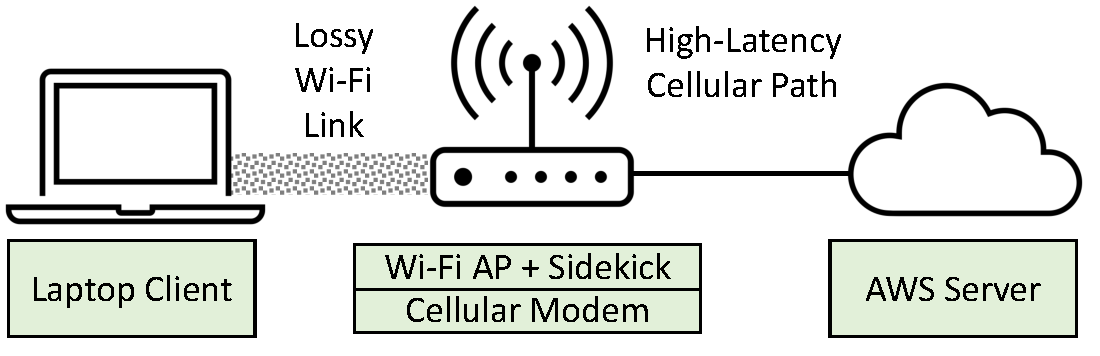
\includegraphics[width=\linewidth]{sidekick-paper/figures/setup_real.pdf}
\caption{Real-world experimental setup.
\vspace{-0.4cm}
}
\label{fig:setup:real}
\end{figure}

\begin{figure*}
% python latencies.py --percentile 99 --box-and-whiskers --http base quack_2p_8 -t 20
% python latencies.py --percentile 99 --box-and-whiskers -t 20
\begin{subfigure}{0.34\textwidth}
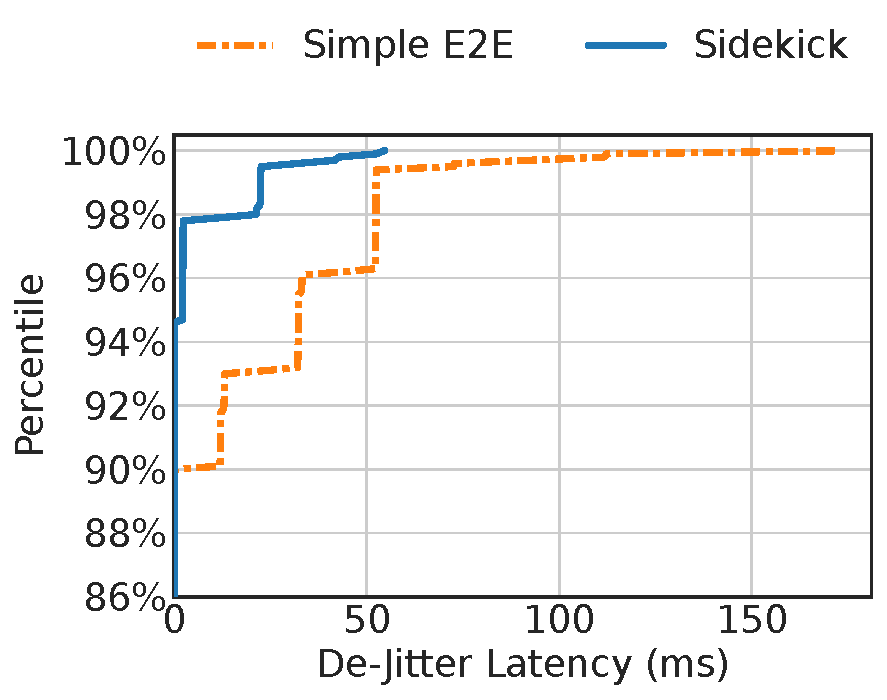
\includegraphics[width=\linewidth]{figures/fig4a_low_latency_media.pdf}
\caption{Scenario \#1: Low-latency media.
 Reduced tail latency of de-jitter delay
with earlier retransmission. 5 minute trials.}
\label{fig:media}
\end{subfigure}
\hfill
% python data_size_vs_tput.py --mean --median -t 10 --http quic quack_30ms_10 quack_60ms_20 quack_120ms_40
% python data_size_vs_tput.py --mean --median -t 10 --http quack_30ms_10 quic
\begin{subfigure}{0.31\textwidth}
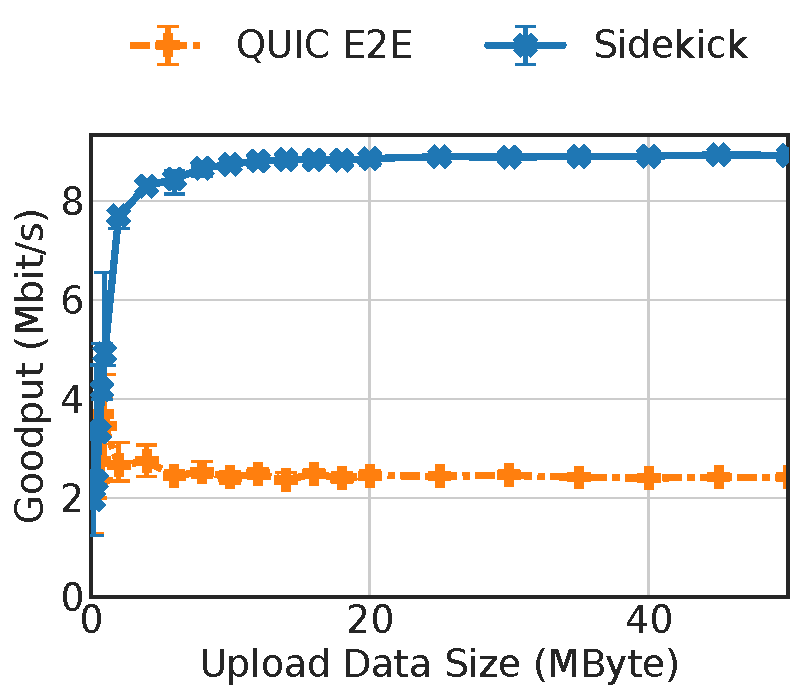
\includegraphics[width=0.97\linewidth]{figures/fig4b_pep_emulation.pdf}
\caption{Scenario \#2: Connection-splitting PEP emulation. Improved goodput.
20 trials median. Error bars are 1st and 3rd quartiles.
}
\label{fig:baseline-line}
\end{subfigure}
\hfill
\begin{subfigure}{0.32\textwidth}
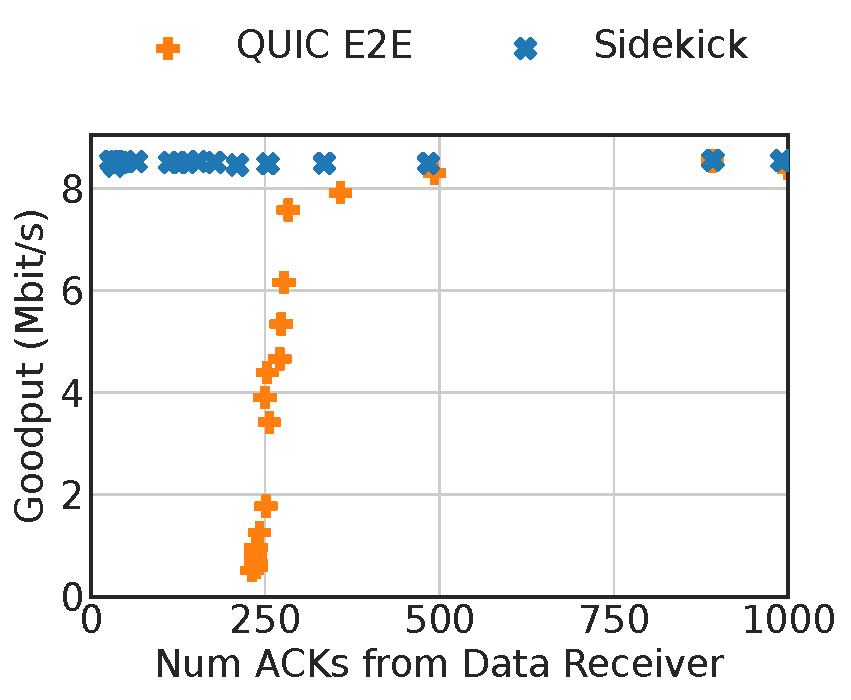
\includegraphics[width=0.99\linewidth]{figures/fig4c_ack_reduction.pdf}
\caption{Scenario \#3: ACK reduction.
High goodput independent of end-to-end ACK frequency.
10 MB upload.}
\label{fig:ack-reduction}
\end{subfigure}
\caption{
Comparing the end-to-end baseline protocol to the same protocol with a \sys
connection, using the success metrics for the three scenarios described in
\Cref{tab:experimental-scenarios}. The \textsf{\Sys($N$x)} data points show
the performance at $N$x the quACK interval (sent less frequently) and
threshold of the default configurations specified in
\Cref{tab:experimental-scenarios}.
\vspace{-0.3cm}
}
% \dm{Maybe a notation like $x/4$ would be more suggestive than $4x$?}
\label{fig:main-results}
\end{figure*}


We evaluated Robin to answer the following questions:
\begin{enumerate}[noitemsep,topsep=0pt]
	\item Can Sidekicks improve the performance of opaque transport protocols
	in a variety of scenarios while preserving the opaque behavior of the
	base protocols?
	\item Can a path-aware congestion control algorithm match the fairness of
	split TCP PEPs using CUBIC?
	\item How do the CPU overheads of encoding quACKs impact the maximum
	capacity of a proxy with a Sidekick?
	\item What link overheads does the power sum quACK add and how does it
	compare to the strawmen?
	\item Is Robin robust in a real-world environment?
\end{enumerate}

\subsection{Methodology}
\label{sec:sidekick:evaluation:methodology}

We modeled the scenarios from \Cref{sec:sidekick:motivating} in both
emulated and real-world environments. We answer questions 1-4 in emulation
and question 5 in the real world. We use the same m4.xlarge AWS instance
as before for the emulated experiments, and as the server in the real-world
experiments.

\paragraph{Emulated environment.}
We emulated a two-hop network topology (\Cref{fig:sc-protocols}) in mininet,
configuring the link properties using \texttt{tc}.
In emulation, we represented
each link by a constant delay (with variability induced by the queue), a random
loss percentage, and a maximum bandwidth.
\Cref{tab:experimental-scenarios} describes the parameters
for each link to model---e.g., lossy Wi-Fi or a high-latency cellular
path---as well as the metrics for success in that scenario.
Link 1 connects the data sender (client) to the proxy,
while Link 2 connects the proxy to the data receiver (server).
On the proxy, we either run a Sidekick,
a connection-splitting TCP PEP~\cite{caini2006pepsal}, or nothing at all.

\paragraph{Real-world environment.}
To test its robustness, we also evaluated Robin over a real-world
environment that resembled the scenario on the train (\Cref{fig:setup:real}).
In this setup, a Lenovo ThinkPad laptop, running Ubuntu 22.04.3 with a 4-Core
Intel i7 CPU @ 2.60 GHz and 16 GB memory, acted as a client to an AWS instance in
the nearest geographical region. The ThinkPad used as an access point (AP)
a Lenovo Yoga laptop, running Ubuntu 20.04.6 with a 4-Core Intel i5 CPU @
1.60 GHz and 4 GB memory, with a 2.4 GHz Wi-Fi hotspot.
The AP was connected to the Internet via a JEXtream cellular modem
with a 5G data plan. The AP ran Sidekick software.

We measured the link properties of each path segment to compare to
our emulation parameters. We measured delay and loss using 1000~\texttt{ping}s
over a 100 second period, and bandwidth using an \texttt{iperf3} test.
On the near segment between the ThinkPad client and the AP,
the min/avg/max/stdev RTT was 1.249/37.194/272.168/54.660 ms
at 49.8 Mbit/s bandwidth. We observed that loss increased
the further away the AP. In our experiments, the client was located roughly
200 feet away in a different room, with 3.6\% loss.
The far segment between the AP and the AWS server was
48.546/64.381/92.374/6.806 ms with 0.0\% loss at 30.9 Mbit/s.
In both environments, the cellular link was the bottleneck link in terms of
bandwidth, and the corresponding path segments in emulation had similar
minimum RTTs and average loss percentages.

\subsection{Main Performance Results}
\label{sec:sidekick:evaluation:main-results}

We first evaluate Robin's main performance goal: In each of the motivating
scenarios, we show that Robin can improve performance compared to the base
protocol alone, which would not be able to benefit from existing PEPs.
Each scenario has a different metric for success---tail latency, throughput,
or number of packets sent by the data receiver (corresponding to energy usage
or chance of Wi-Fi collisions)---demonstrating the versatility of the Sidekick
protocol.

\paragraph{Low-Latency Media.}
The Sidekick can reduce tail latencies in a low-latency media stream, representing
fewer drops and better quality of experience.
The early retransmissions induced by the Sidekick reduced the 99th percentile
latency of the de-jitter buffer delay from 48.6 ms to 2.2 ms---a 95\%
reduction (\Cref{fig:media}).
As long as the quACK interval is less than the end-to-end RTT, the connection
benefits from the Sidekick.

The Sidekick is beneficial in this scenario because it enables the client to sooner
detect and retransmit lost packets, and the server to sooner play packets from
its de-jitter buffer.
The end-to-end mechanism takes one additional received packet to notify of the
loss and
one end-to-end RTT to retransmit and play the packet (20+52=72ms), resulting in
three delayed packets (the three ``steps" in \Cref{fig:media}) in most cases.
The Sidekick takes up to two additional packets and one near path segment RTT
(20+2=22ms or 20$\times$2+2=42ms), delaying either one or two packets in comparison.
Dropped ACKs and quACKs account for the $<2\%$ of packets with even greater
de-jitter latencies.

\paragraph{Connection-Splitting PEP Emulation.}
The Sidekick improves upload speeds when there is a lossy, low-latency link
by using quACKs to inform the sender's congestion control.
In a scenario with $1\%$ random loss on the link between the proxy and the
data sender, the HTTP/3 (QUIC) client achieves $3.6\times$ the goodput for a 10 MB
upload with a Sidekick compared to end-to-end QUIC (\Cref{fig:baseline-line}).

When there is no random loss, the Sidekick does not impact the performance
of QUIC\@.
There are no logical changes to the base protocol in this case because all loss
is on the
bottleneck link on the far path segment, and the CPU overheads of processing quACKs
are negligible.

Knowing \emph{where} congestion occurs is an opportunity for creating smarter
congestion control. In PACUBIC, identifying where the loss occured let the data
sender reduce the congestion window proportionally to how many packets were
in-flight on each path segment. In \Cref{sec:sidekick:evaluation:pacubic}, we
will show that our path-aware congestion control algorithm still matches the
fairness of connection-splitting TCP PEPs.

\paragraph{ACK Reduction.}

Using quACKs in lieu of end-to-end ACKs allows the data receiver to
significantly reduce its ACK frequency while maintaining high goodput.
In our experiment, QUIC with a Sidekick sent $96\%$ fewer packets (mainly ACKs)
than end-to-end QUIC before the goodput dropped below 8.5 Mbit/s
(\Cref{fig:ack-reduction}).
The quACK enables the data sender to promptly move the flow-control window forward,
as long as the last hop is reliable.

The goodput significantly degrades when reducing the end-to-end ACK frequency
without a Sidekick. When end-to-end QUIC reduces the ACK frequency to every
80 ms, the data receiver sends $247 / 138 = 1.8\times$ the packets at
$4.5 / 8.4 = 0.5\times$ the goodput, worse than QUIC with the Sidekick
in both dimensions (\Cref{fig:ack-reduction}). With a Sidekick,
the data sender also does not need to change packet pacing to avoid bursts in
response to infrequent ACKs, which is why end-to-end QUIC cannot send fewer
than $\approx 240$ packets.

\subsubsection{Configuring the Sidekick Connection}
\Cref{tab:experimental-scenarios} shows the quACK interval and threshold we
elected for each scenario based on the considerations in
\Cref{sec:sidekick:protocol}. In each experiment in \Cref{fig:main-results},
we also show how with less frequent quACKs ($2\times$ and $4\times$ the
interval) and proportionally-adjusted thresholds, the protocol performs worse,
or more variably. Less frequent quACKs means the client reacts later to
feedback about the near path segment, and more often has to rely on the
end-to-end mechanism. The performance particularly degrades when the quACK
interval exceeds the end-to-end RTT. However, even in this case, the base
protocol with any Sidekick at all performs better than the base protocol alone\@.

\subsection{Link Overheads}
\label{sec:sidekick:evaluation:link-overheads}

\begin{figure}[h]
\begin{subfigure}{\columnwidth}
  % 5+
  %
  \setlength{\tabcolsep}{2pt}
  \footnotesize
  \centering
  \begin{tabular}{lccccccc}
    \toprule
    & \multicolumn{2}{c}{Data Sender$\rightarrow$} & \multicolumn{2}{c}{$\leftarrow$Proxy} & \multicolumn{2}{c}{$\leftarrow$Data Receiver} & \\
    & \bf Pkts & \bf Bytes & \bf Pkts & \bf Bytes & \bf Pkts & \bf Bytes & \bf Goodput \\
    \midrule
    QUIC E2E & $1.00\times$ & $1.00\times$ & $1.00\times$ & $1.00\times$ & $1.00\times$ & $1.00\times$ & $1.00\times$ \\
    Strawman 1a & $0.96\times$ & $1.01\times$ & \cellcolor{LighterRed}{$2.02\times$} & \cellcolor{LightestRed}{$1.56\times$} & $1.01\times$ & $1.03\times$ & \cellcolor{LighterGreen}{$3.33\times$} \\
    Strawman 1b & $0.94\times$ & $1.00\times$ & \cellcolor{LighterRed}{$2.00\times$} & \cellcolor{LightestRed}{$1.78\times$} & $1.00\times$ & $1.03\times$ & \cellcolor{LightGreen}{$3.53\times$} \\
    Strawman 1c & \cellcolor{LightestRed}{$1.83\times$} & $1.06\times$ & \cellcolor{LighterRed}{$2.01\times$} & \cellcolor{LightestRed}{$1.83\times$} & $1.00\times$ & $1.03\times$ & \cellcolor{LightGreen}{$3.46\times$} \\
    \bf \textcolor{black!50!blue}{Power Sum}   & \textcolor{black!50!blue}{\bf 0.94$\times$} & \textcolor{black!50!blue}{\bf 1.00$\times$} & \textcolor{black!50!blue}{\bf 1.03$\times$} & \textcolor{black!50!blue}{\bf 1.07$\times$} & \textcolor{black!50!blue}{\bf 1.00$\times$} & \textcolor{black!50!blue}{\bf 1.03$\times$} & \cellcolor{LightGreen}{\textcolor{black!50!blue}{\bf 3.55$\times$}} \\
    \bottomrule
  \end{tabular}
  % \includegraphics[width=\columnwidth]{figures/packet-overhead-retx.png}
  \caption{Scenario \#2: Connection-splitting PEP emulation.}
  \label{tab:packet-overhead:retx}
\end{subfigure}
\begin{subfigure}{\columnwidth}
  % \includegraphics[width=\columnwidth]{figures/packet-overhead-ackr.png}
  \setlength{\tabcolsep}{2pt}
  \footnotesize
  \centering
  \begin{tabular}{lccccccc}
    \toprule
    & \multicolumn{2}{c}{Data Sender$\rightarrow$} & \multicolumn{2}{c}{$\leftarrow$Proxy} & \multicolumn{2}{c}{$\leftarrow$Data Receiver} & \\
    & \bf Pkts & \bf Bytes & \bf Pkts & \bf Bytes & \bf Pkts & \bf Bytes & \bf Goodput \\
    \midrule
    QUIC E2E & $1.00\times$ & $1.00\times$ & $1.00\times$ & $1.00\times$ & $1.00\times$ & $1.00\times$ & $1.00\times$ \\
    Strawman 1a & $0.96\times$ & $1.00\times$ & \cellcolor{LightRed}{$9.94\times$} & \cellcolor{LighterRed}{$4.99\times$} & \cellcolor{LightGreen}{$0.04\times$} & \cellcolor{LightGreen}{$0.08\times$} & $1.02\times$ \\
    Strawman 1b & $0.96\times$ & $1.00\times$ & \cellcolor{LightRed}{$9.95\times$} & \cellcolor{LightRed}{$7.13\times$}      & \cellcolor{LightGreen}{$0.04\times$} & \cellcolor{LightGreen}{$0.08\times$} & $1.02\times$ \\
    Strawman 1c & \cellcolor{LightestRed}{$1.91\times$} & $1.05\times$ & \cellcolor{LightRed}{$9.73\times$} & \cellcolor{LightRed}{$7.41\times$}      & \cellcolor{LightGreen}{$0.04\times$} & \cellcolor{LightGreen}{$0.08\times$} & $0.97\times$ \\
    \bf \textcolor{black!50!blue}{Power Sum}    & \textcolor{black!50!blue}{\bf 0.96$\times$} & \textcolor{black!50!blue}{\bf 1.00$\times$} & \textcolor{black!50!blue}{\bf 1.09$\times$} & \cellcolor{LighterRed}{\textcolor{black!50!blue}{\bf 2.56$\times$}} & \cellcolor{LightGreen}{\textcolor{black!50!blue}{\bf 0.04$\times$}} & \cellcolor{LightGreen}{\textcolor{black!50!blue}{\bf 0.08$\times$}} & \textcolor{black!50!blue}{\bf 0.98$\times$} \\
    \bottomrule
  \end{tabular}
  \caption{Scenario \#3: ACK reduction.}
  \label{tab:packet-overhead:ackr}
\end{subfigure}
\caption{Link overheads for a 10 MB upload. The cells represent the multiplier
relative to the end-to-end QUIC baseline for each type of quACK\@.
Lower is better for number of packets and bytes sent on a link.
Higher goodput is better. Robin's power sum quACK achieves the success metric
for each scenario without incurring the link overheads of the strawmen.
We did not evaluate the contrived protocol in Scenario \#1.
}
\label{tab:packet-overhead}
\end{figure}


The other cost in terms of using Sidekick protocols is the additional data
sent by the proxy to the data sender.
Too many additional bytes use up bandwidth, and additional packets use
up CPU\@.
\Cref{tab:packet-overhead} shows the number of packets and bytes sent at each
node comparing the strawmen and power sum quACK to no Sidekick connection at all.

Using power sum quACKs increases the packets sent from the proxy to the data
sender
by 3-9\%. These packets either consist mostly
of end-to-end ACKs which are sent every packet in \texttt{quiche}, or end-to-end
ACKs that have been replaced by quACKs in the ACK reduction scenario.
We did not evaluate Scenario \#1 because it is based
on a contrived protocol that lacks many of these features, and the link
overheads would not really make sense.

This overhead is representative of the CPU overhead at the client, since
quACKs and ACKs take a similar number of cycles to process. In an experiment
with Scenario \#2 during a period of $\approx90$k incoming packets, ACKs took on
average 26065 cycles to process while the quACKs took 26369 cycles, 1\% more.
These cycles come from, i.e., the complex recovery and loss detection algorithms
implemented at the end host.

The strawmen have significantly higher link overheads compared to the power sum
quACK\@. The proxy sends up to 10$\times$ more packets using Strawman 1a, and
also slightly harms the goodput in the congestion control scenario.
The reduced goodput is due to the sender mis-identifying received packets as
dropped due to dropped quACKs.
The proxy achieves higher goodput with Strawman 1b but sends
more bytes. Strawman 1c increases the link overheads at both the proxy and the
data sender due to larger TCP headers and TCP ACKs.
We did not evaluate Strawman 2 due to its impractical decode time.

\subsection{CPU Overheads}
\label{sec:sidekick:evaluation:cpu-overheads}

\begin{table}[ht]
  \centering
  \small
  \begin{tabular}{lrrrr}
    \toprule
    & \multicolumn{2}{r}{\bf 25-Byte Payload} & \multicolumn{2}{r}{\bf 1468-Byte Payload}\\
    & \bf Cycles & \bf $\%$ & \bf Cycles & \bf $\%$ \\
    \midrule
    Sniff Packet & 22417 & 97.6 & 22408 & 97.5 \\
    Table Lookup &   247 &  1.1 &   251 &  1.1 \\
    Parse ID     &    23 &  0.1 &    22 &  0.1 \\
    Encode ID    &    74 &  0.3 &    69 &  0.3 \\
    Other        &   213 &  0.9 &   225 &  1.0 \\
    \midrule
    \emph{Total} & \emph{22974} & \emph{100.0} & \emph{22975} & \emph{100.0} \\
    \bottomrule
  \end{tabular}
  \caption{Breakdown of the CPU cycles spent processing each packet at the
  proxy. Most cycles are spent on general per-packet overheads as opposed to
  quACK-specific processing.
  }
  \label{tab:cpu-overhead}
\end{table}


The main bottleneck of Robin on a proxy is the CPU\@.
\Cref{tab:cpu-overhead} shows a breakdown of the number of CPU cycles in each
step. The largest overhead was reading the packet contents from the network
interface ($97.5\%$ of the CPU cycles).

Encoding an identifier in a power sum quACK with $t=10$ used $74$ CPU
cycles ($0.9\%$). As a calculation of the theoretical maximum on a 2.30 GHz
% 2.30e9 / 74 = 31 million
CPU, the proxy would be able to process $31$ million packets/second on a single
core. The hash table lookup used $251$ cycles and parsing the pseudorandom
payload as an identifier used $22$ cycles.

In practice, we measured the maximum throughput of Robin to
be 464k packets/s with 25-byte payloads and 5.5 Gbit/s (458k packets/s) with
1468-byte packet payloads on a single core (assuming 1500-byte MTUs).
This experiment used multiple \texttt{iperf3} clients to simulate high
load until Robin was unable to keep up with the load on a single core.
The packet payload size did not seem to affect results.

We find these achieved throughputs acceptable for edge routers such as Wi-Fi
APs and base stations.
To deploy Robin on core routers, we would need to reduce the overhead of reading
packets from the NIC, such as by bypassing the kernel/user-space
protection boundary\footnote{
A kernel-bypass system like Retina~\cite{wan2022retina} can achieve
25 Gbps on 2 cores while processing raw packets with a 1000-cycle callback
(Figure 5(a) in \cite{wan2022retina}). The Sidekick equivalent would be a 500-cycle
callback, and assuming all traffic has requested Sidekick help. Throughput scales
almost linearly with the number of cores using symmetric RSS hashing.
Thus we don't expect proxy overheads to be an issue with modern 100 Gbps network
speeds and an optimized implementation even on commodity hardware.
}~\cite{dpdk,mccanne1993bsd,wan2022retina}
or using native hardware~\cite{bosshart2014p4}.
We could also scale on multiple cores using symmetric RSS hashing~\cite{woo2012scalable}.

\subsection{Path-Aware CUBIC}
\label{sec:sidekick:evaluation:pacubic}

\begin{figure}[t]
\centering
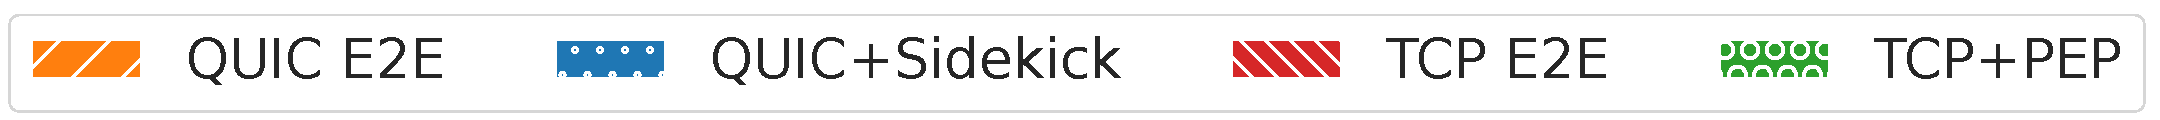
\includegraphics[width=\columnwidth]{figures/fig5_baseline_bar_legend.pdf}
\begin{subfigure}{0.49\linewidth}
	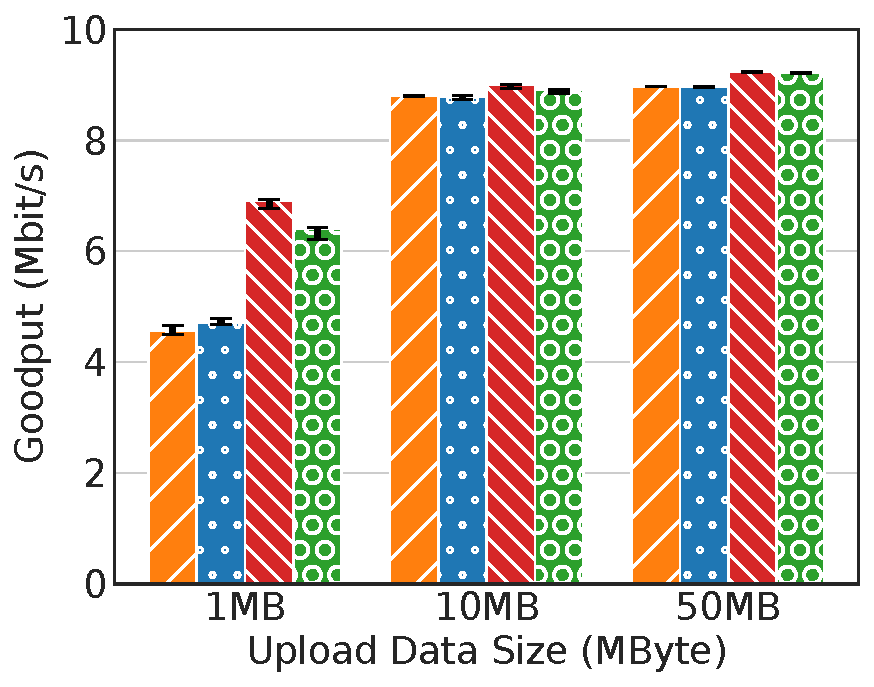
\includegraphics[width=\linewidth]{figures/fig5_baseline_loss0p.pdf}
	\caption{0\% loss.}
	\label{fig:baseline-bar:loss0p}
\end{subfigure}
\begin{subfigure}{0.49\linewidth}
	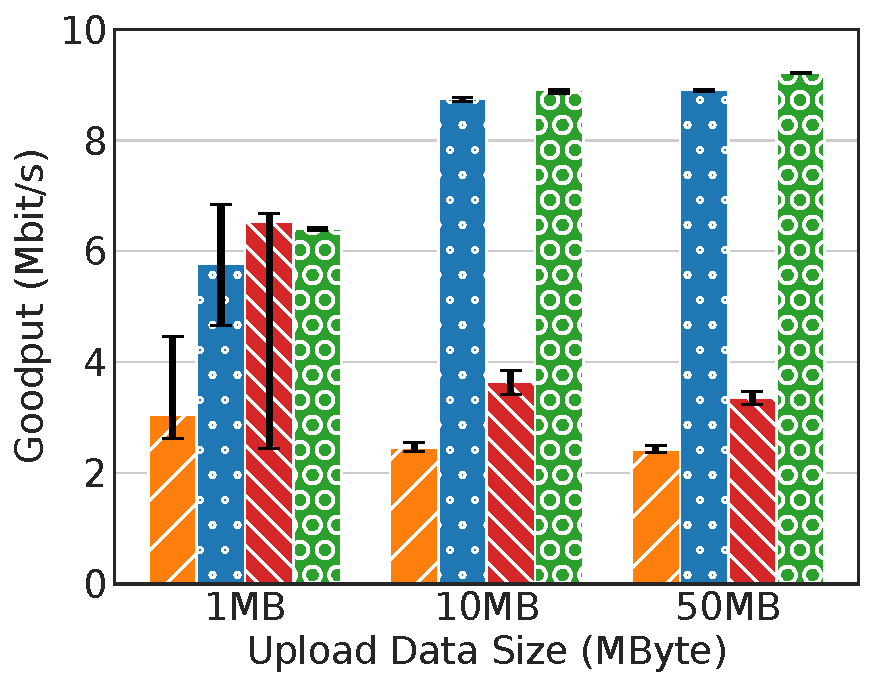
\includegraphics[width=\linewidth]{figures/fig5_baseline_loss1p.pdf}
	\caption{1\% loss.}
	\label{fig:baseline-bar:loss1p}
\end{subfigure}
\vspace{-0.2cm}
\caption{Median goodput for three upload data sizes with $0\%$ and $1\%$ loss on
Link 1. 20 trials. Error bars are 1st and 3rd quartiles.
With proxy assistance at $1\%$
loss, both QUIC and TCP match the performance of when there is no loss at all.
\vspace{-0.4cm}
}
\label{fig:baseline-bar}
\end{figure}

\begin{figure}[t]
\centering
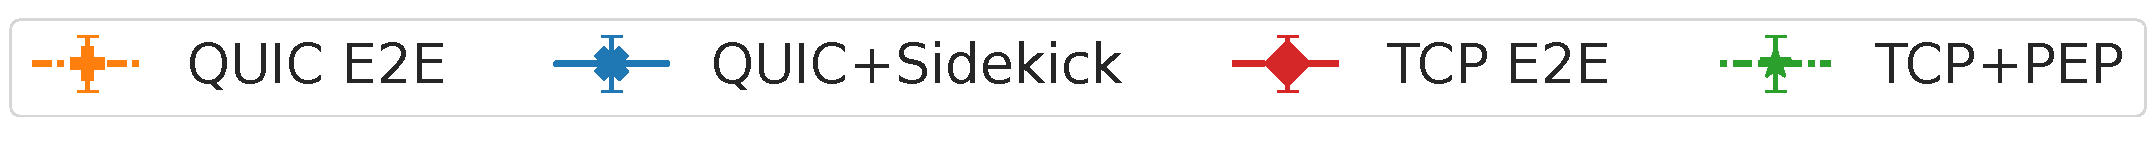
\includegraphics[width=\columnwidth]{figures/fig6_legend.pdf}
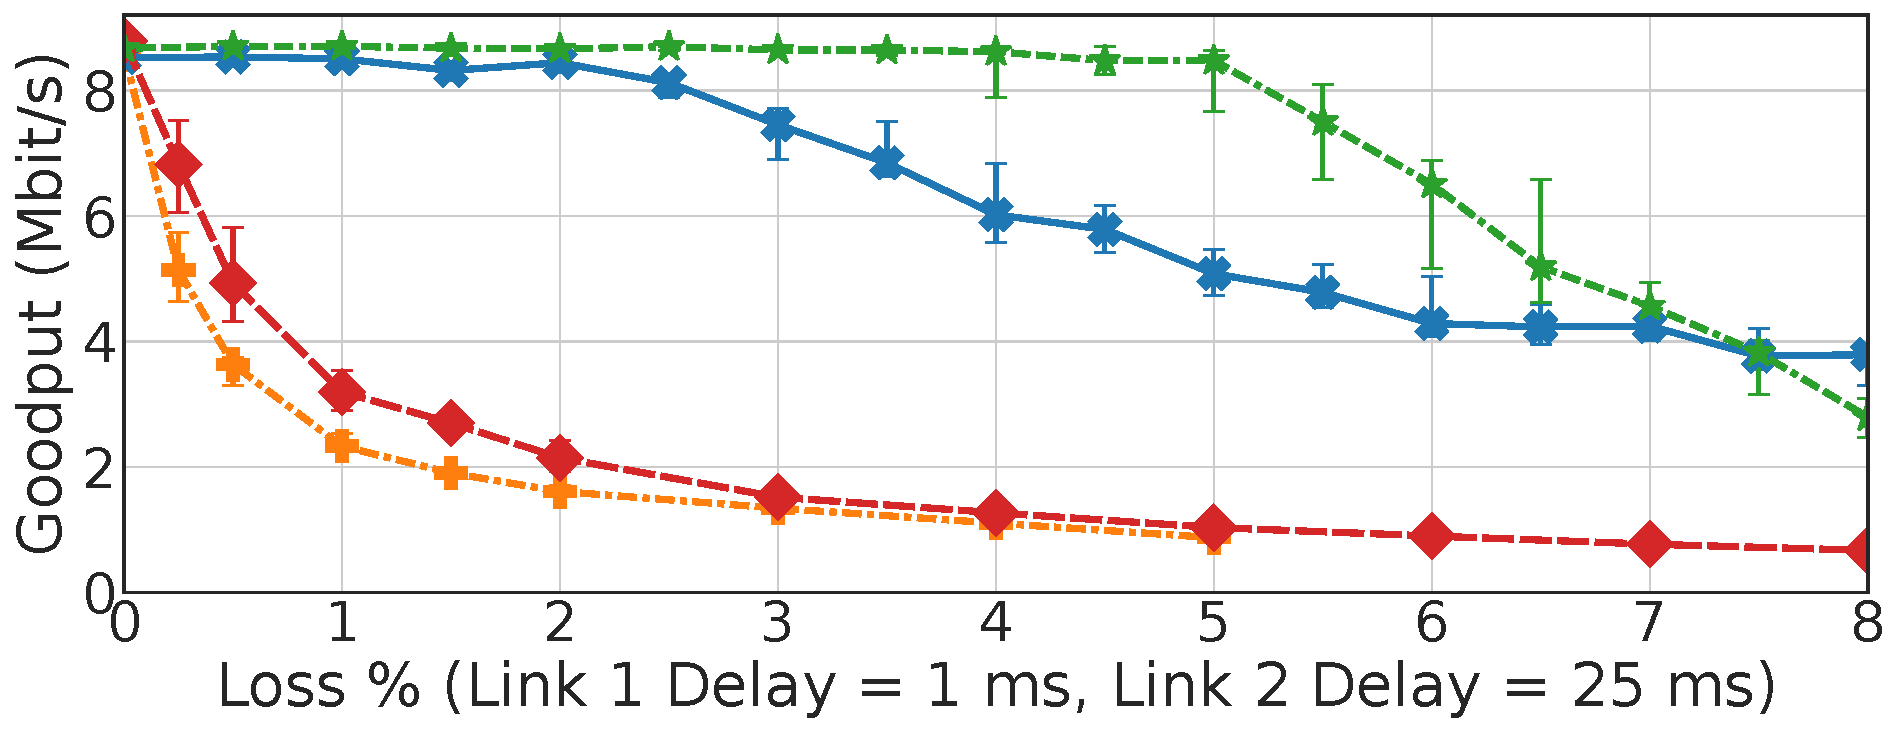
\includegraphics[width=\columnwidth]{figures/fig6_loss_bw100_10M_delay_25ms_1ms.pdf}
%\includegraphics[width=\columnwidth]{figures/loss_bw100_10M_delay_15ms_11ms.pdf}
\vspace{-0.4cm}
\caption{Connection-splitting PEP emulation as a function of near-segment
	loss rate. In this emulation experiment, QUIC+\Sys (running PACUBIC)
  performs similarly to TCP+PEP (each connection running CUBIC)
  and improves goodput compared with end-to-end protocols. The graph shows
  median goodput of a 10~MByte upload. QuACK interval is 30~ms, threshold
is 10. Error bars show IQR of 10 trials.
\vspace{-1cm}
}
\label{fig:loss-vs-tput}
\end{figure}

%\begin{figure}[t]
%\centering
%	\includegraphics[width=0.6\linewidth]{figures/multiflow_loss0p_legend.pdf}\\
%	\includegraphics[width=0.32\linewidth]{figures/quic_quack_60M_loss0p_delay0s_bw100.pdf}
%	\includegraphics[width=0.32\linewidth]{figures/quic_quack_60M_loss0p_delay5s_bw100.pdf}
%	\includegraphics[width=0.32\linewidth]{figures/quack_quic_60M_loss0p_delay5s_bw100.pdf}
%        \caption{Fairness evaluation of two concurrent QUIC flows in
%          Scenario \#1 (but without loss on the near path segment), one \sys-assisted and one end-to-end, in a purely
%          congestion-limited situation. The use of
%          \sys assistance doesn't affect 
%
%          Throughput of two concurrent flows in Scenario 1 (with $0\%$ and $1\%$
%loss on Link 1. Both flows converge to a steady-state throughput, whether the
%flows start at the same time (left) or at a 5 second delay (middle, right).}
%\label{fig:multiflow}
%\end{figure}

% \begin{figure*}
% \centering
% \includegraphics[width=\columnwidth]{figures/legend.pdf}\\
% \subfigure[QUIC, QUIC no delay]{
% 	\includegraphics[width=0.185\textwidth]{figures/quic_quic_60M_loss0p_delay0s.pdf}
% 	\label{fig:multiflow:a}}
% \subfigure[QUIC, QUIC 5s delay]{
% 	\includegraphics[width=0.185\textwidth]{figures/quic_quic_60M_loss0p_delay5s.pdf}
% 	\label{fig:multiflow:b}}
% \subfigure[QUIC, \sys no delay]{
% 	\includegraphics[width=0.185\textwidth]{figures/quic_quack_60M_loss0p_delay0s.pdf}
% 	\label{fig:multiflow:c}}
% % \subfigure[quack, quic no delay]{
% % 	\includegraphics[width=0.185\textwidth]{figures/quack_quic_60M_loss0p_delay0s.pdf}}
% \subfigure[QUIC, \sys 5s delay]{
% 	\includegraphics[width=0.185\textwidth]{figures/quic_quack_60M_loss0p_delay5s.pdf}
% 	\label{fig:multiflow:d}}
% \subfigure[\sys, QUIC 5s delay]{
% 	\includegraphics[width=0.185\textwidth]{figures/quack_quic_60M_loss0p_delay5s.pdf}
% 	\label{fig:multiflow:e}}
% % \label{fig:multiflow:quic-quack}
% % \end{figure*}

% % \begin{figure*}
% % \centering
% \subfigure[PEP, PEP no delay]{
% 	\includegraphics[width=0.185\textwidth]{figures/pep_pep_60M_loss1p_delay0s.pdf}
% 	\label{fig:multiflow:f}}
% \subfigure[PEP, PEP 5s delay]{
% 	\includegraphics[width=0.185\textwidth]{figures/pep_pep_60M_loss1p_delay5s.pdf}
% 	\label{fig:multiflow:g}}
% \subfigure[PEP, \sys no delay]{
% 	\includegraphics[width=0.185\textwidth]{figures/pep_quack_60M_loss1p_delay0s.pdf}
% 	\label{fig:multiflow:h}}
% % \subfigure[quack, pep no delay]{
% % 	\includegraphics[width=0.185\textwidth]{figures/quack_pep_60M_loss1p_delay0s.pdf}}
% \subfigure[PEP, \sys 5s delay]{
% 	\includegraphics[width=0.185\textwidth]{figures/pep_quack_60M_loss1p_delay5s.pdf}
% 	\label{fig:multiflow:i}}
% \subfigure[\sys, PEP 5s delay]{
% 	\includegraphics[width=0.185\textwidth]{figures/quack_pep_60M_loss1p_delay5s.pdf}
% 	\label{fig:multiflow:j}}
% \caption{Multiflow experiment with various combinations of QUIC end-to-end and QUIC+\sys at 0\% loss (a-e),
% and various combinations of TCP+PEP and QUIC+\sys at 1\% loss (f-j), demonstrating
% flow fairness. The delay indicates how long we started the second flow after the first flow.}
% \label{fig:multiflow}
% \end{figure*}


It is easy to improve performance without regard to competing flows;
however, we demonstrate that PACUBIC can
match the fairness of split CUBIC in a TCP PEP connection\@.
We evaluate fairness using Scenario \#2 with varying amounts of loss on the
near path segment.

\paragraph{QUIC vs.\ TCP\@.}
We first compare QUIC to TCP without either PEP\@.
As both connections use CUBIC, they exhibit similar
congestion control behavior and achieve nearly maximum throughput in the
emulated network with no random loss (\Cref{fig:baseline-bar:loss0p}).
We attribute the differences to the slightly different retranmission and
loss recovery behaviors of QUIC and TCP\@. The PEPs do not affect the
performance.

With even a little loss on the near path segment, both QUIC and TCP dramatically
worsen, respectively achieving $28\%$ and $42\%$ of the goodput at $0\%$ loss,
for a 10 MB upload (\Cref{fig:baseline-bar:loss1p}).
% 0.305 / 1.098 = 27.8%
% 0.467 / 1.121 = 41.7%
In both protocols, CUBIC treats every transmission error as a congestion event,
even though no amount of reducing the congestion window affects the error rate.
QUIC and TCP perform similarly to each other with proxy assistance and 1\%
loss on the near path segment.

\paragraph{Sidekick vs.\ TCP PEP\@.}
\Cref{fig:loss-vs-tput} shows that QUIC with a Sidekick roughly matches---as
 intended---the behavior of TCP with a PEP-assisted split connection. At higher
loss rates, the near path segment becomes the bottleneck link even with earlier
feedback about loss, causing the performance of TCP with proxy assistance to
drop. QUIC with a Sidekick follows a similar pattern because of its path-aware
congestion-control scheme (\Cref{sec:sidekick:protocol:sender-behavior}). The
results indicate that the Sidekick protocol's gains do not come at the expense
of congestion-control fairness relative to the split TCP connection.

\section{Real-World Experiments}
\label{sec:sidekick:evaluation:real-world}

\begin{figure}[t]
\centering
\begin{subfigure}{0.48\linewidth}
	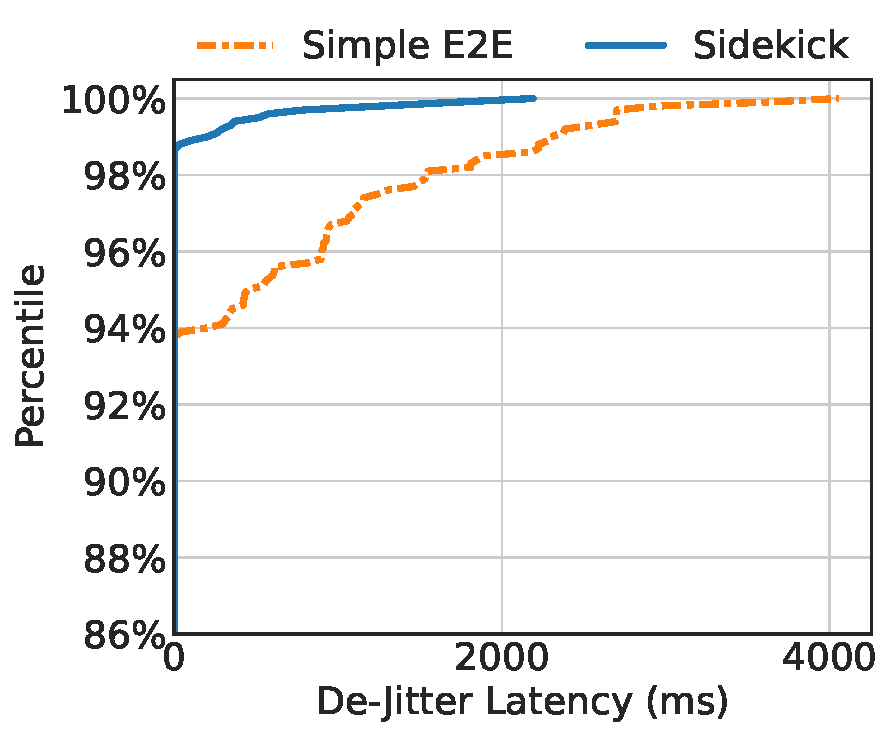
\includegraphics[width=\linewidth]{sidekick-paper/figures/fig8_real_world_webrtc.pdf}
	\caption{\footnotesize Low-latency media. CDF of per-packet de-jitter
	latencies over 10 one-minute trials per protocol.}
	\label{fig:real-world:scenario1}
\end{subfigure}
\begin{subfigure}{0.48\linewidth}
	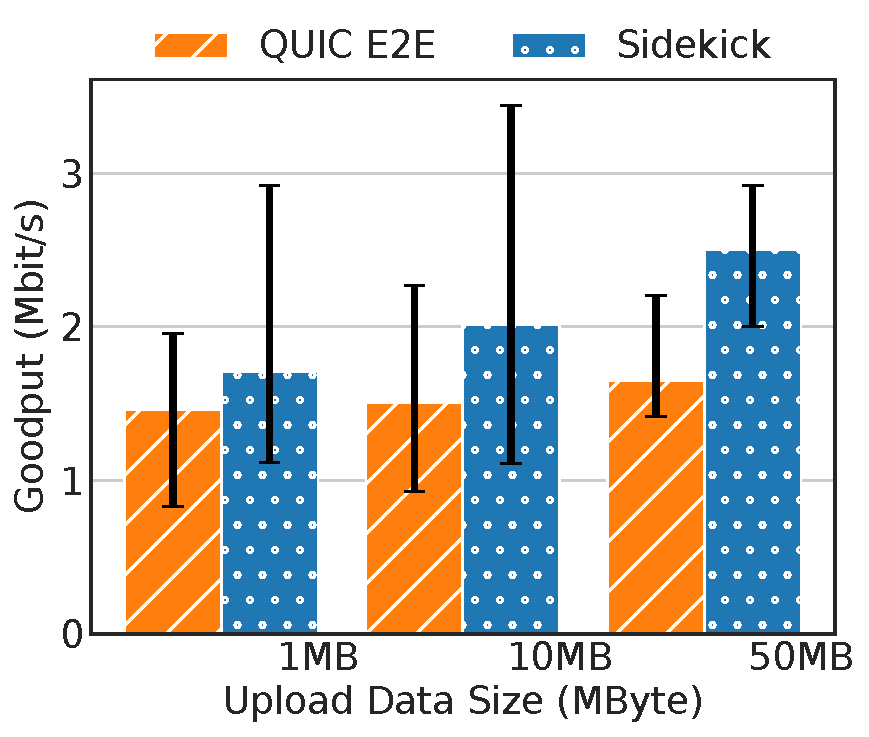
\includegraphics[width=\linewidth]{sidekick-paper/figures/fig8_real_world_retx.pdf}
	\caption{\footnotesize Path-aware congestion control.
	Median of 20 trials. Error bars are 1st and 3rd quartiles.}
	\label{fig:real-world:scenario2}
\end{subfigure}
\caption{Real-world results. Experiments were run in a moderately well-attended
office environment over a Friday afternoon. Trials alternate between the
baseline and the sidekick to account for variability in time of day.
}
\label{fig:real-world}
\end{figure}


We discuss the results of our experiments replicating two of our scenarios in
the real world, using as context
these main differences between emulation and the real-world:

\begin{itemize}[noitemsep,topsep=0pt]
	\item The RTT is more variable as it depends on interactions in the
	wireless medium and the shared cellular path.
	\item Wireless loss can be more variable as nearby 2.4 GHz devices and
	physical barriers may interfere with the link. Wireless loss also tends
	to be more clustered in practice.
	\item The available bandwidth on the shared cellular path is more variable,
	and depends on the time of day.
\end{itemize}

\Cref{fig:real-world} shows the results of running the low-latency media and
connection-splitting PEP emulation experiments in the real-world. The baseline
protocol with a Sidekick is able to
reduce the 99th percentile de-jitter latency of an audio stream
from 2.3~seconds to 204~ms---about a 91\% reduction---and
improve the goodput of a 50 MB HTTP/3 upload by about 50\%.
Although the improvements are more conservative compared to emulation in
\Cref{fig:media} and \Cref{fig:baseline-line}, each case still benefits the
base protocol under all circumstances, compared to end-to-end mechanisms alone.

Part of the difference can be attributed to the network setting. When there is
no loss on the near path segment, as can occasionally happen in a real Wi-Fi link,
we do not expect to
see a difference with a Sidekick. When there is more loss on the far path segment, which
is variable and depends on the time, we
expect the benefit of the Sidekick to be less since this equally affects the
performance of the base protocol.

The other part of the difference could be made up by future work that better
adapts a Sidekick connection to real-world variability: The client could improve
path segment RTT estimation based on when the proxy receives packets, and use this
dynamic estimate in the calculation of $r$ used in $\beta$ and $C$.
The client could also use
this estimate to dynamically adjust the quACK interval.
Finally, we could analyze theoretically how PACUBIC responds
to traffic patterns in the real world.
